\documentclass[a4paper,11pt]{article}
\usepackage[utf8]{inputenc}
\usepackage{graphicx}
\usepackage{geometry}
\usepackage{array}
\usepackage{booktabs}
\usepackage{hyperref}
\usepackage{xcolor}
\usepackage{tikz}
\usepackage{caption}
\usepackage{float}
\usepackage{graphicx}
\geometry{margin=2.5cm}
\hypersetup{
    colorlinks=true,
    linkcolor=black,
    urlcolor=blue
}
\setlength{\parskip}{6pt}
\setlength{\parindent}{0pt}

\usepackage{fancyhdr}
\pagestyle{fancy}
\fancyhf{}
\rfoot{\thepage}

\begin{document}

\begin{center}
    {\LARGE \textbf{Datasheet TS741}}\\
    \vspace{4pt}
    \textit{Distorsore analogico per chitarra\\Progetto sviluppato dal team studentesco \textbf{PoliTeK} – Politecnico di Torino}\\
    \vspace{4pt}
    \rule{\linewidth}{0.5pt}
\end{center}

\section{Overview}
Il TS741 è un pedale distorsore analogico progettato per chitarristi che cercano un suono morbido e dinamico. Si ispira al Tube Screamer, ma presenta modifiche per migliorare la risposta in frequenza e la trasparenza del tono.

\section{Functional Description}

\begin{table}[h!]
    \centering
    \begin{tabular}{|p{0.2\linewidth}|p{0.7\linewidth}|}
        \hline
        \textbf{Controllo} & \textbf{Descrizione} \\
        \hline
        Gain & Regola la quantità di distorsione agendo sul guadagno dello stadio operazionale. \\
        \hline
        Tone & Filtro attivo che enfatizza o attenua le medie frequenze. \\
        \hline
        Level & Regola il volume d’uscita complessivo del pedale. \\
        \hline
    \end{tabular}
    \caption*{Tabella 3 – Descrizione dei controlli}
\end{table}

\section{Features}

\begin{table}[h!]
    \centering
    \begin{tabular}{|p{0.4\linewidth}|p{0.5\linewidth}|}
        \hline
        \textbf{Caratteristica} & \textbf{Descrizione} \\
        \hline
        Controlli & Gain, Tone, Level \\
        \hline
        Bypass & True bypass (footswitch meccanico 3PDT) \\
        \hline
        Clipping & Soft clipping con diodi al silicio, BJT configurati a diodo o LED in controreazione \\
        \hline
        Alimentazione & 9V DC \\
        \hline
        Switch & Per scegliere tra due stadi di clipping differenti \\
        \hline
        PCB & Doppia faccia, progettazione personalizzata \\
        \hline
    \end{tabular}
    \caption*{Tabella 1 – Caratteristiche principali del pedale}
\end{table}

\section{Electrical Specifications}

\begin{table}[H]
    \centering
    \begin{tabular}{|l|l|}
        \hline
        \textbf{Parametro} & \textbf{Valore Tipico} \\
        \hline
        Tensione di alimentazione & 9V DC \\
        \hline
        Assorbimento di corrente & XXX \\
        \hline
        Impedenza di ingresso & XXX \\
        \hline
        Impedenza di uscita & XXX \\
        \hline
        Risposta in frequenza & XXX \\
        \hline
    \end{tabular}
    \caption*{Tabella 2 – Specifiche elettriche}
\end{table}

\section{Frequency response}
Inserire poi foto

\section{Clipping Characteristic}
Inserire poi foto

\section{Schematic diagram}

\begin{figure}[H]
    \centering
    \includegraphics[width=1\textwidth]{images/ts9_modificato.png}
    \caption{Schematic of the circuit}
    \label{fig:schematic}
\end{figure}

L'alimentazione è garantita dallo stadio Power Supply che in ingresso accetta i 9 V DC, mentre il segnale segue il seguente percorso:

\begin{center}
    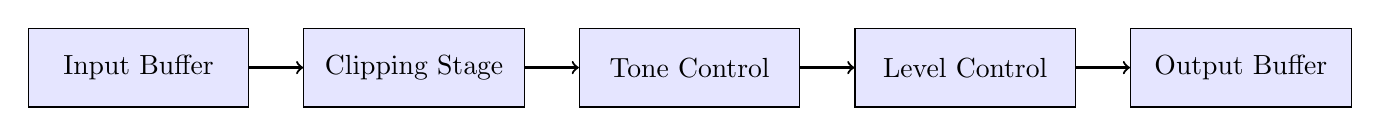
\begin{tikzpicture}[node distance=3.5cm, auto, every node/.style={draw, fill=blue!10, minimum height=1cm, minimum width=2.8cm}]
        \node (in) {Input Buffer};
        \node[right of=in] (gain) {Clipping Stage};
        \node[right of=gain] (tone) {Tone Control};
        \node[right of=tone] (level) {Level Control};
        \node[right of=level] (out) {Output Buffer};
        \draw[->, thick] (in) -- (gain);
        \draw[->, thick] (gain) -- (tone);
        \draw[->, thick] (tone) -- (level);
        \draw[->, thick] (level) -- (out);
    \end{tikzpicture}
\end{center}

\section{PCB layout}
Inserire poi foto

\section{Connectors and Layout}

\begin{itemize}
    \item \textbf{Input Jack:} Audio jack 6,35 mm – da chitarra
    \item \textbf{Output Jack:} Audio jack 6,35 mm – verso amplificatore
    \item \textbf{Alimentazione:} esterna tramite DC Barrel jack 2,1 mm o tramite batteria
\end{itemize}

\section{Key Components}

\begin{table}[h!]
    \centering
    \renewcommand{\arraystretch}{1.2}
    \begin{tabular}{|l|p{10cm}|}
        \hline
        \textbf{Componente} & \textbf{Modello} \\
        \hline
        OpAmp & TL072 – JFET low-noise dual op-amp \\
        \hline
        Diodi di Clipping & 1N4148 e 1N4004 (diodi al silicio), OA95 (diodi al germanio), LED e transistor configurati a diodo \\
        \hline
        Condensatori & Film e elettrolitici \\
        \hline
        Footswitch & 3PDT – true bypass \\
        \hline
        \end{tabular}
    \caption*{Tabella 4 – Componenti principali}
\end{table}    

\section{Mechanical dimensions}
Bhoo

\section{Notes and Recommendations}

\begin{itemize}
    \item Non superare i 9V in ingresso.
    \item Usare alimentatori stabilizzati per evitare rumore.
    \item Collegare prima l'alimentazione, poi lo strumento.
\end{itemize}

\section{Contact and Credits}

Per info o supporto:
\begin{itemize}
    \item link github se rendiamo la repo pubblica
\end{itemize}

\end{document}